\section{System Architecture}
\label{sec:architecture}

CircuitCraft is built on Fabric, a lightweight, widely used modding toolchain for
Minecraft. The codebase is organized into five packages, shown in
Figure~\ref{fig:architecture}: a solver package with no dependency on any Minecraft class at
all, a pair of packages describing the in-world blocks and their per-block simulation
state, a networking/topology package that ties placed blocks together into a circuit and
synchronizes probe readings to clients, and a client-only package responsible for rendering
the oscilloscope heads-up display.

\begin{figure}[htbp]
\centering
\begin{tikzpicture}[
    box/.style={draw, rounded corners, minimum width=6.2cm, minimum height=1cm,
                align=center, font=\small},
    node distance=0.45cm
]
\node[box, fill=gray!10] (sim) {\texttt{sim} --- pure-Java MNA circuit solver\\(no Minecraft dependency)};
\node[box, below=of sim, fill=blue!8] (blockentity) {\texttt{blockentity} --- per-block simulation state\\(components, wire/ground nodes, modules)};
\node[box, below=of blockentity, fill=blue!8] (block) {\texttt{block} --- placement, orientation, right-click interaction};
\node[box, below=of block, fill=orange!12] (network) {\texttt{network} --- topology construction, solve loop,\\multi-channel probe protocol};
\node[box, below=of network, fill=green!10] (client) {\texttt{client} --- oscilloscope HUD rendering (client-side only)};

\draw[-{Latex[length=2mm]}] (blockentity) -- (sim);
\draw[-{Latex[length=2mm]}] (block) -- (blockentity);
\draw[-{Latex[length=2mm]}] (network) -- (blockentity);
\draw[-{Latex[length=2mm]}] (network) -- (sim);
\draw[-{Latex[length=2mm]}] (client) -- (network);
\end{tikzpicture}
\caption{Package-level architecture. The solver has zero Minecraft dependencies and is
directly unit-testable with plain \texttt{javac}/\texttt{java}; every other layer builds on
it.}
\label{fig:architecture}
\end{figure}

\subsection{Components and topology}

A two-terminal component occupies a single block, oriented along the horizontal or vertical
axis the player was facing when it was placed; its two electrical leads are its front and
back faces along that axis, and its other four faces are electrically insulated. Which of the
four figures below a given block appears in (Sections~\ref{sec:circuit-elements}
through~\ref{sec:probes}) depends only on its electrical role -- element, topology-only,
source, or measurement tool -- not on any special-casing in the topology algorithm itself,
which treats all seventeen blocks and items uniformly.

Once per game tick, for each independent group of adjacent, mutually-conductive blocks
(a ``network''), the mod rebuilds a union--find partition over every block face that
presents a conductive surface toward a conductive neighbor, assigns one MNA node index to
each resulting partition, and instructs every component in that network to stamp itself
into the circuit between its resolved node indices.

The ideal op-amp (Section~\ref{sec:circuit-solver}) is the mod's first component with three
electrical leads rather than two, which the topology algorithm above accommodates without
any per-terminal-count branching: the union--find partitioning already keys each block face
independently on whether the entity it belongs to is a single shared node (as wire and
ground are) or a distinct lead, so an entity simply exposes as many independently keyed
leads as it has terminals, and the final node-resolution step reads off however many
resolved indices that entity declared, whether two or three.

\subsection{Circuit elements}
\label{sec:circuit-elements}

Figure~\ref{fig:elements} shows the six elements a circuit's topology is actually built
from: the resistor, capacitor, and inductor (Section~\ref{sec:circuit-solver} gives each
element's transient stamp, Section~\ref{sec:ac-analysis} its AC admittance), the memristor
(Section~\ref{sec:related-work}), the diode, and the ideal op-amp, the mod's only
three-terminal component (see above). A plain right-click cycles each through a small set of
preset values; the shift-right-click value editor (Section~\ref{sec:limitations}) additionally
accepts an arbitrary value directly for every element except the diode (a categorical
silicon/germanium/LED choice) and the op-amp (fixed, ideal behavior with no adjustable
parameter at all).

\begin{figure*}[!t]
\centering
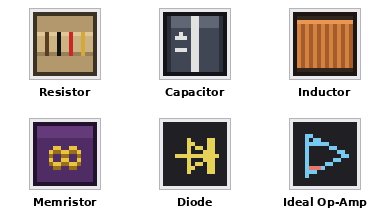
\includegraphics[width=0.6\textwidth]{figures/elements_gallery.png}
\caption{The six circuit elements: resistor, capacitor, inductor, memristor, diode, and ideal
op-amp.}
\label{fig:elements}
\end{figure*}

\subsection{Wire and ground}

Figure~\ref{fig:wireground} shows the mod's only two purely topological blocks. A wire
conducts on all six faces and has no orientation of its own; a ground block (see
Section~\ref{sec:circuit-solver}) behaves identically to wire for topology purposes but
additionally establishes the network's voltage reference, so that every other node's solved
voltage is meaningful as an absolute quantity rather than only relative to some other probed
point. Both are placed and removed with no adjustable state at all.

\begin{figure}[htbp]
\centering
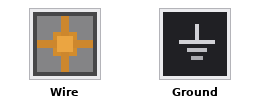
\includegraphics[width=0.28\textwidth]{figures/wire_ground_gallery.png}
\caption{Wire and ground, the mod's only two purely topological blocks.}
\label{fig:wireground}
\end{figure}

\subsection{Generators}

Figure~\ref{fig:generators} shows the mod's three independent voltage sources, plus the two
modules that adjust one of them. The power supply is a fixed-DC source stepped through a
preset voltage cycle; the function generator produces a sine, square, or triangle wave
(cycled by right-click) at a default 5~V, 1~Hz, overridden independently by a voltage module
or a frequency module placed directly against one of its side faces -- these are the
function generator's ``additional elements,'' each a single-purpose block with no function of
its own beyond feeding one number to whichever generator it is attached to. The AC Source
(Section~\ref{sec:ac-analysis}) is not a transient source at all: it contributes nothing to
the regular per-tick simulation and exists solely to be swept by the AC probe
(Section~\ref{sec:probes} below), its amplitude and frequency range set entirely through the
value editor rather than a preset cycle. All three sources -- power supply, function
generator, and AC Source alike -- additionally require a redstone signal before they drive
anything at all (Section~\ref{sec:pedagogy} discusses the pedagogical reasoning): the first
two remain an open circuit, and the AC Source sweeps silently at 0~V, until powered.

\begin{figure*}[!t]
\centering
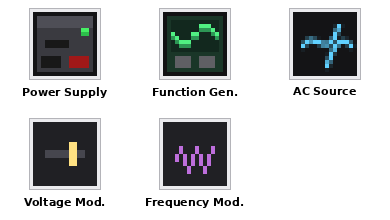
\includegraphics[width=0.6\textwidth]{figures/generators_gallery.png}
\caption{The three voltage sources -- power supply, function generator, and AC Source -- and
the two modules, voltage and frequency, that adjust the function generator's output.}
\label{fig:generators}
\end{figure*}

\subsection{Probes}
\label{sec:probes}

Figure~\ref{fig:probes} shows the mod's four measurement tools. The ammeter is the odd one
out: an in-circuit block rather than a handheld item, wired in series like any other
two-terminal component, electrically an ideal 0~V source (a wire) so it reports an exact
branch current with no series resistance to distort whatever it is measuring. The other three
are handheld items a player holds rather than places -- the time-domain oscilloscope probe,
the X-Y probe, and the AC (Bode-plot) probe -- each pinned against components, wires, or
ground blocks to read them rather than wired into the network itself, described in their own
subsections below and in Section~\ref{sec:ac-analysis} respectively.

\begin{figure}[htbp]
\centering
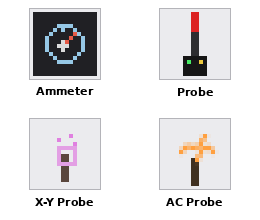
\includegraphics[width=0.4\textwidth]{figures/probes_gallery.png}
\caption{The four measurement tools: the in-circuit ammeter, and three handheld oscilloscope
probes.}
\label{fig:probes}
\end{figure}

\subsection{Multi-channel oscilloscope protocol}

A handheld probe item allows a player to pin up to three components, wires, or ground
blocks simultaneously (a right-click pins an object or promotes it to most-recently-used
status; shift-right-click unpins it). The server streams each pinned position's
instantaneous voltage, current, a 200-sample rolling history, and a short human-readable
summary to that player once per tick, and the client renders each of the up to three
channels as an independently color-coded, auto-scaled oscilloscope trace stacked in a
corner of the screen, as shown in Figure~\ref{fig:scope}, with each trace's own full-scale
value printed at the top and bottom of its graph in whichever SI-prefixed form (kilo, milli,
micro, nano, or pico) keeps the printed number compact. A component's trace displays the
voltage drop across its two leads (or, for the ammeter, the branch current, reusing the
same history and rendering machinery so that current and voltage may be observed side by
side without a separate ``current channel'' concept); a wire or ground block's trace
displays its single node's absolute voltage relative to whatever ground reference the
network possesses, discussed in the following section. Once all three channel slots are
occupied, the oldest pinned channel is outlined and labeled to show which channel the next
pin would evict, so a player deciding whether to add a fourth signal can see the consequence
of that choice before committing to it, rather than discovering which trace disappeared only
after the fact.

\subsection{The X-Y oscilloscope probe}

A second, independent probe item allows a player to pin exactly two channels and view them
plotted against one another rather than against time: one channel's voltage on the
horizontal axis, the other's on the vertical axis, the same X-Y display mode a real bench
oscilloscope provides. Pinning is append-only with a two-slot cap: whichever position was
just right-clicked -- new or already pinned -- always becomes the more recently pinned of
the two, which unconditionally assigns it to the vertical (Y) axis, demoting the previous Y
to X and, if both slots were already occupied, evicting the previous X entirely.

Each axis is scaled independently to its own channel's peak magnitude, rather than sharing a
single scale, so that two signals of very different size -- a few volts on one channel,
millivolts on the other -- each still occupy the plot's full range instead of one being
compressed to a sliver by the other's larger scale; the two independent full-scale values are
printed at both extremes of each axis, directly on the plot, again in whichever SI-prefixed
form keeps the number compact. This does not sacrifice the shared-scale
case's original benefit: a shape only has a distorted aspect ratio when the two channels'
peak magnitudes genuinely differ, so two equal-amplitude sinusoids in quadrature still trace
an actual circle rather than a stretched ellipse, since their independently computed scales
necessarily coincide. This mode is pedagogically distinct from the time-domain probe: it
makes the relative phase and amplitude between two signals directly visible as a shape,
rather than requiring a player to compare two scrolling traces by eye.
